
We would like to generalize the sorting problem. What if, when sorting a set of
elements, we already had some information on the order of these elements?


It is clear that we could use this information to ease the overall computation
process. If we look at any \BigO{\text{ITLB}} algorithm, they all start from
$0$ bits of information and end up producing a totally ordered set containing
$\text{ITLB}~= n \log n$ bits of information. We already shown in
\ref{tree:sorting:ITLB} that for any algorithm, there exists an instance of the
problem wich will force the algorithm to ask \BigOmega{n \log n} questions.
Starting from a poset whose order is completely unknown, such an algorithm will
thus iteratively update this poset by retrieving information and make sure it
reuses it well. By reusing the information efficiently, it will be able to
choose ``good'' questions to ask.


In quicksort this is achieved by recursively building linear extensions of weak
orders. In weak orders, elements of a poset are layered in sets of incomparable
elements (maximum cardinality stable sets) that are disjoint from each other.
Thus quicksort will never have to ask a question about elements from disjoint
sets. However, the way quicksort chooses questions doesn't guarantee that every
step of the algorithm will evenly divide stable sets. In conclusion, while
quicksort can sometimes ask poor quality questions, it also reuses information
it has optimally.


We take as a second example the algorithm mergesort. Mergesort works by
iteratively merging totally ordered sets $P$ and $Q$, and for the sake of
simplicity we consider that those sets have the same cardinality $n$  (in
reality their cardinalities can only differ by $1$). We saw in
\ref{tree:merging:k=2} that each of these steps can be computed with an
algorithm whose complexity is \BigO{n}. For each merge operation, the input
contains $2n \log n$ bits of information while the output contains $2n \log 2n$
bits of information, so we must find $2n \log 2n - 2n \log n = 2n (\log n +
\log 2 - \log n) = 2n$ bits of information, which is consitant with our
previous results. So, regarding reuse of retrieved information the mergesort
algorithm is optimal.

\begin{figure} \centering \begin{subfigure}[b]{0.4\textwidth}
{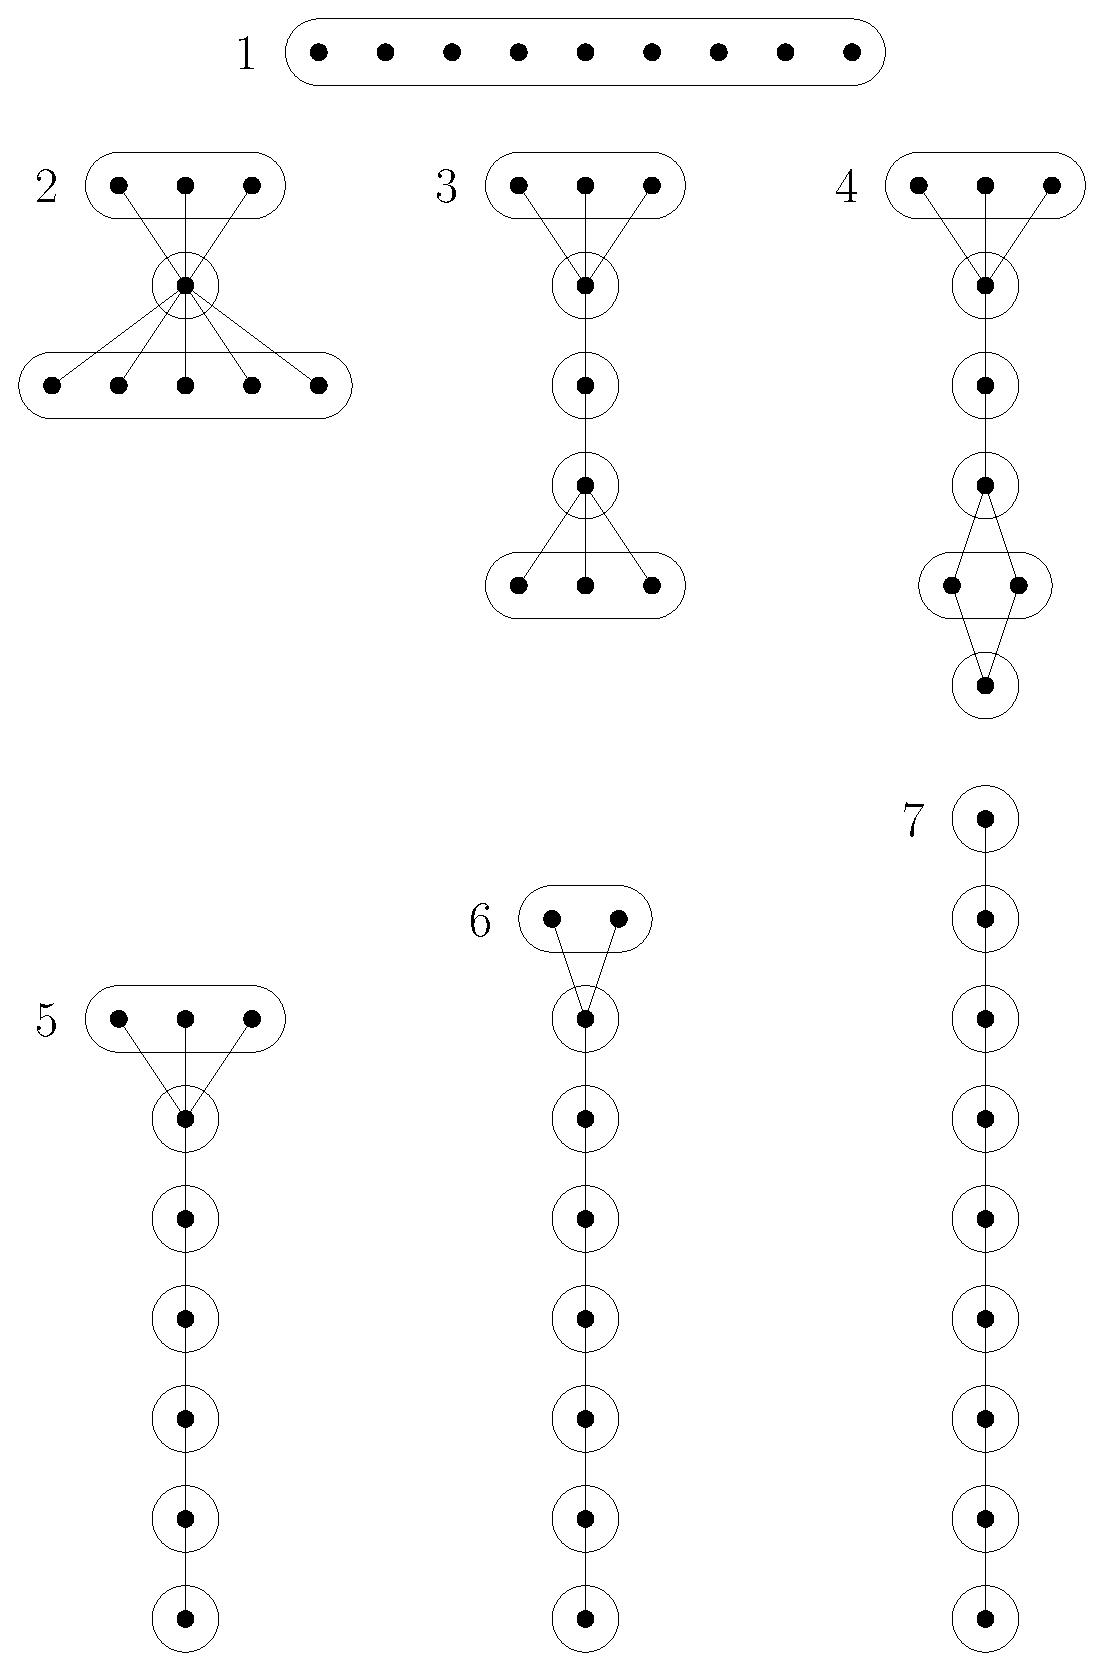
\includegraphics[width=\textwidth]{fig/supi/quicksort}} \caption{Steps of the
quicksort algorithm represented as Hasse diagrams (maximal antichains / stable
sets are circled).} \label{fig:supi:quicksort} \end{subfigure}
\begin{subfigure}[b]{0.4\textwidth}
{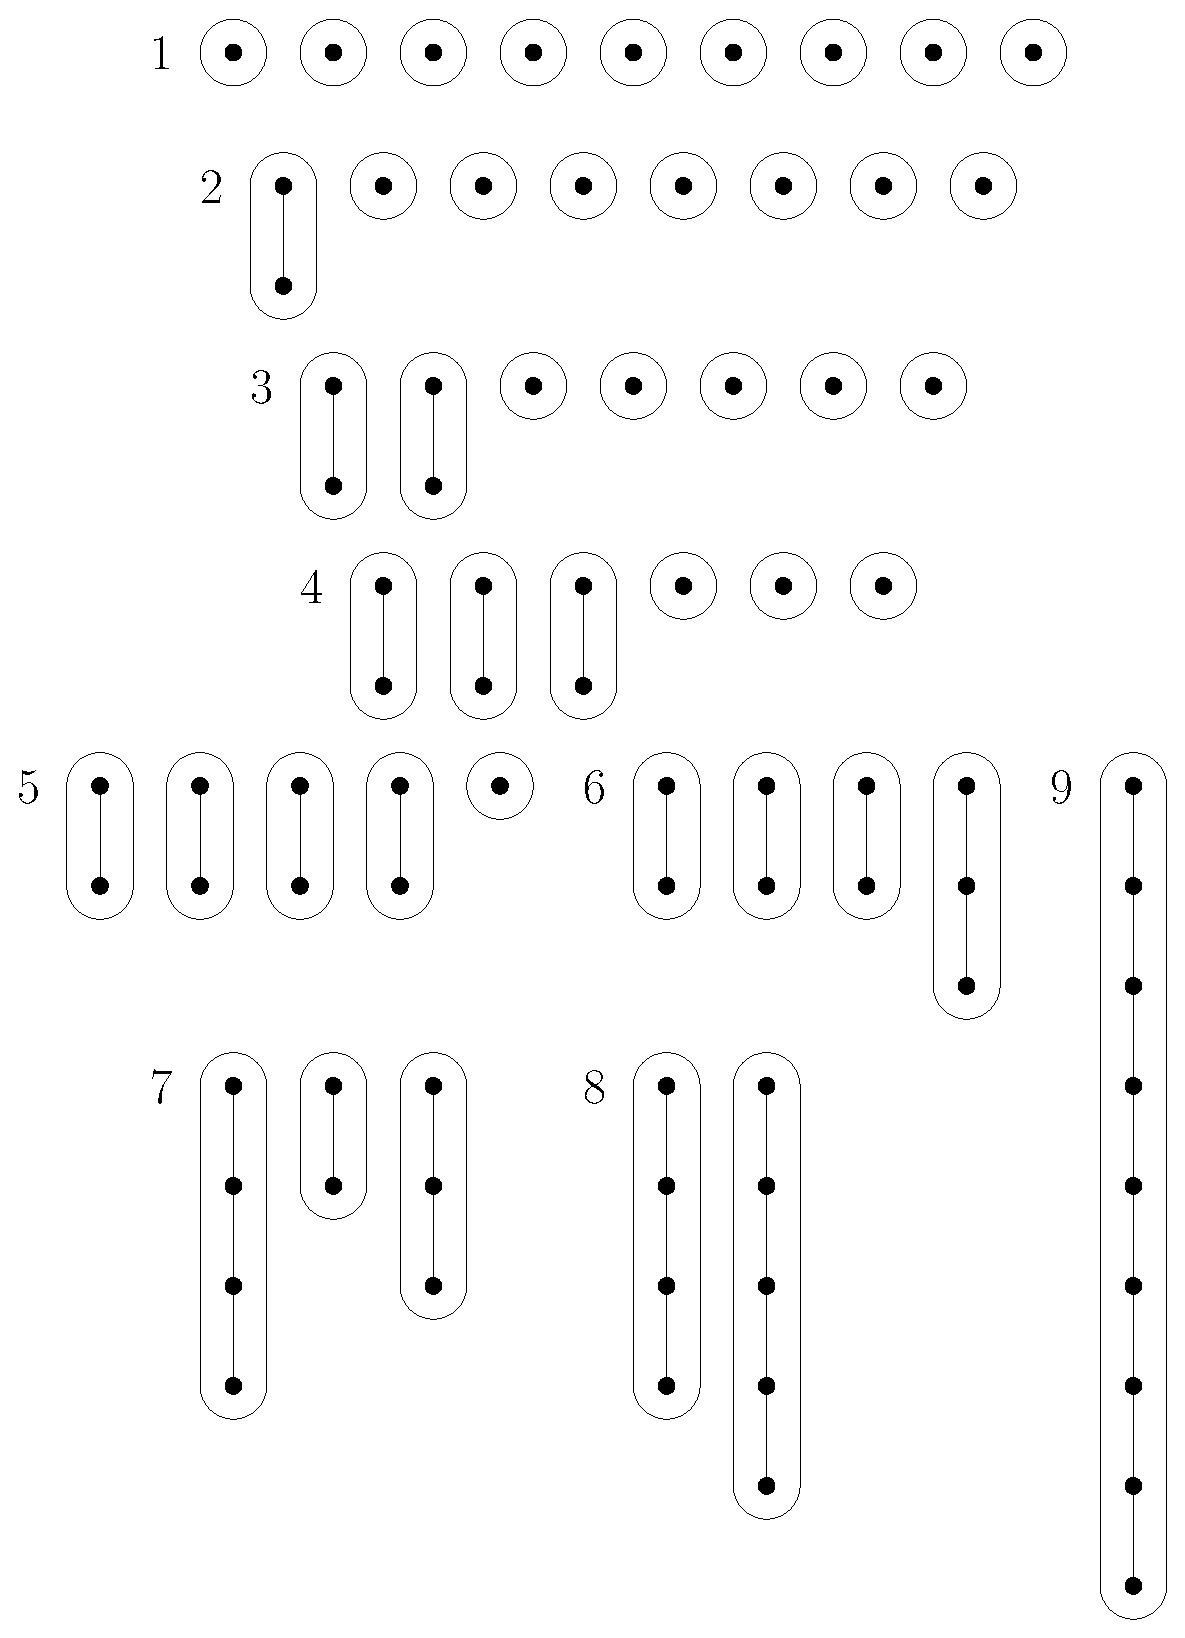
\includegraphics[width=\textwidth]{fig/supi/mergesort}} \caption{Steps of the
mergesort algorithm represented as Hasse diagrams (maximal chains / cliques are
circled).} \label{fig:supi:mergesort} \end{subfigure} \end{figure}


\cref{fig:supi:quicksort,fig:supi:mergesort} show the iterative poset
generation processes of a run of quicksort and mergesort. They sum up what we
observed about those algorithms, that they only work on a particular subset of
posets.

What we will be interested in this chapter are algorithms that can sort any
poset (not just those handled by classical sorting algorithms) optimally with
respect to the number of comparisons.
